\section{1174057 Alit Fajar Kurniawan}
    \subsection{Teori}
   		\begin{enumerate}
   			\item Jelaskan kenapa kata-kata harus di lakukan vektorisasi
   			\par Alasan mengapa kata-kata harus dilakukan vektorisasi terlebih dahulu yaitu dikarenakan mesin hanya mampu membaca data dengan bentuk angka. Berdasarkan hal tersebut maka tentunya diperlukan vektorisasi kata atau bisa disebut dengan mengubah kata menjadi bentuk vektor agar mesin seolah-olah paham apa yang kita maksudkan dan dapat memproses aktifitas/perintah dengan benar. Kata juga harus di vektorisasi untuk mengetahui presentase kata yang sering muncul dalam setiap kalimatnya, yang berguna untuk menetukan kata kunci. 
   			\begin{figure}[H]
				\centering
				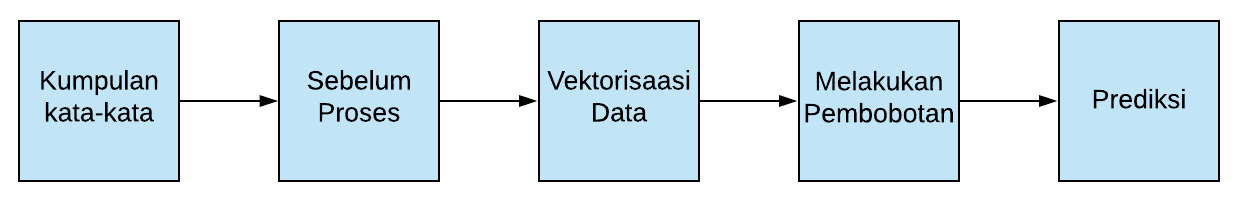
\includegraphics[scale=0.5]{figures/1174057/chapter5/1.png}
				\caption{Vektorisasi Kata}
				\label{Vektorisasi Kata}
			\end{figure}

			\item Jelaskan mengapa dimensi dari vektor dataset google bisa sampai 300
			\par Dimensi dari Vektor Dataset Google Bisa Mencapai 300 itu dikarenakan pada masing-masing objek yang terdapat pada dataset akan memiliki identitasnya tersendiri, selain itu juga untuk nilai dalam vektor 300 dimensi yang terkait dalam sebua kata ”dioptimalkan” dalam berbagai hal untuk menangkap aspek yang berbeda dari makna dan penggunaan kata itu. Apabila dicontohkan dengan penjelasan yang lebih rinci maka dilakukan perumpamaan sederhana. Misalnya untuk sebuah dataset google yang memiliki 3 buah objek yaitu berat, lebar, dan tinggi. Kemudian dari masing-masing objek tersebut dilakukan perbandingan antara berat dan lebar beserta berat dan tinggi. Hasil yang didapatkan akan memiliki presentasi yang berbeda sehingga dapat diartikan bahwa mesin dapat membedakan objek yang hampir serupa namun tak sama. 
			\begin{figure}[H]
				\centering
				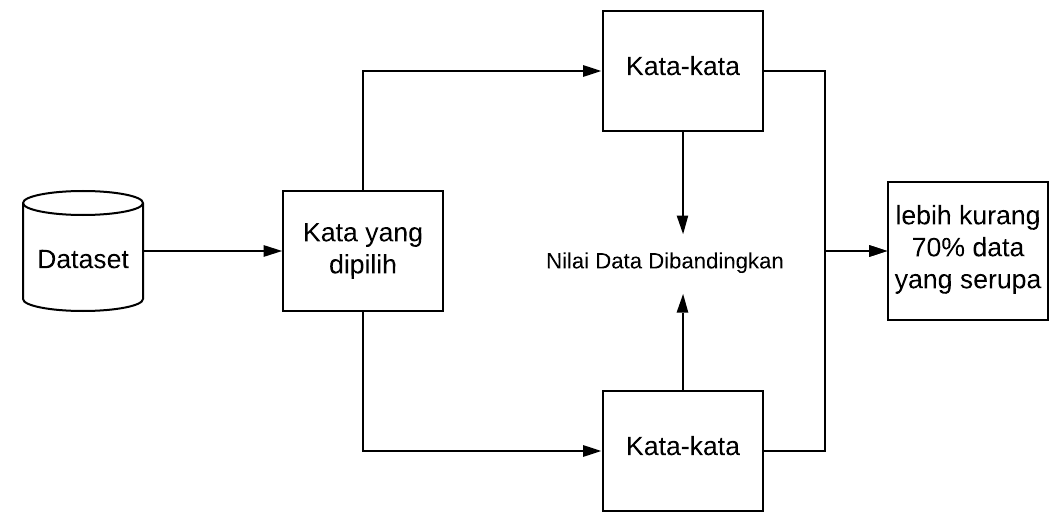
\includegraphics[scale=0.4]{figures/1174057/chapter5/2.png}
				\caption{Dataset Google}
				\label{Dataset Google}
			\end{figure}

			\item Jelaskan konsep vektorisasi untuk kata
			\par Konsep untuk vektorisasi kata sebenarnya sama dengan ketika dilakukan input suatu kata pada mesin pencarian. Kemudian untuk hasilnya akan mengeluarkan ( berupa ) referensi mengenai kata tersebut. Jadi data kata tersebut didapatkan dari hasil pengolahan pada kalimat-kalimat sebelumnya yang telah diolah. misalnya pada kalimat berikut (Belajar Kecerdasan buatan Poltekpos), pada kalimat tersebut terdapat konteks yakni poltekpos, kata tersebut akan dijadikan data latih untuk mesin yang akan dipelajari dan diproses. Jadi ketika kita inputkan kata poltekpos, maka mesin akan menampilkan keterkaitannya dengan kata tersebut sehingga akan lebih efisien dan lebih mudah. 
			\begin{figure}[H]
				\centering
				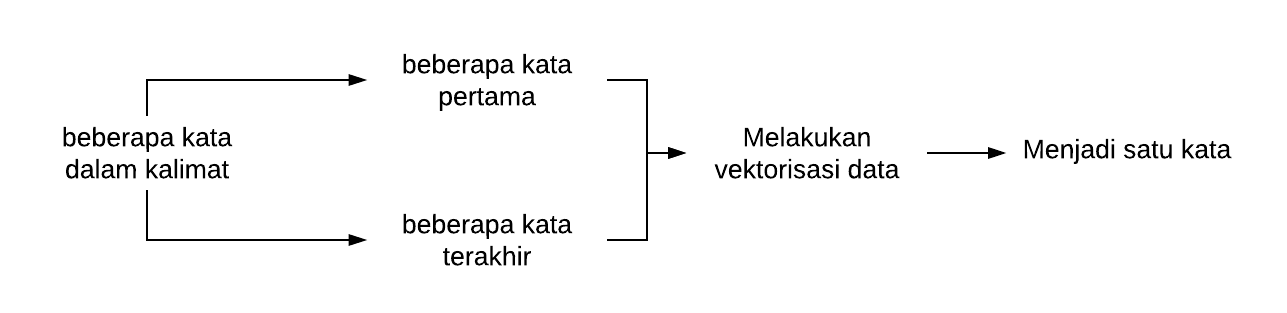
\includegraphics[scale=0.4]{figures/1174057/chapter5/3.png}
				\caption{konsep vektorisasi}
				\label{konsep vektorisasi}
			\end{figure}

			\item Jelaskan konsep vektorisasi untuk dokumen
			\par Untuk vektorisasi dokumen sebenarnya terbilang sama dengan konsep vektorisasi kata, yang membedakan hanya pada proses awalnya. Untuk vektorisasi dokumen ini, mesin akan membaca semua kalimat yang terdapat pada dokumen tersebut, kemudian kalimat yang terdapat pada dokumen tersebut akan di pecah menjadi kata-kata
			\begin{figure}[H]
				\centering
				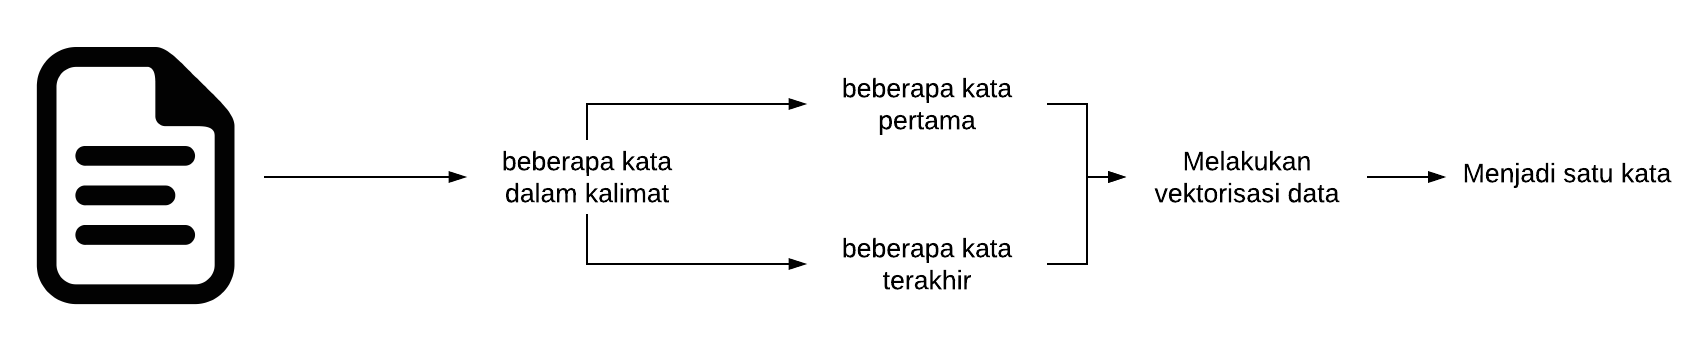
\includegraphics[scale=0.4]{figures/1174057/chapter5/4.png}
				\caption{konsep vektorisasi Dokumen}
				\label{konsep vektorisasi Dokumen}
			\end{figure}

			\item Jelaskan apa mean dan standar deviasi
			\par Mean merupakan nilai rata-rata dari suatu data. Mean sendiri dapat dicari dengan cara membagi jumlah data dengan banyak data sehingga diperoleh lah nilai rata-rata dari suatu data yang dicari sedangkan standar deviasi sendiri merupakan sebuah teknik statistik yang digunakan dalam menjelaskan homogenitas kelompok ataupun dapat diartikan dengan nilai statistik dimana dimanfaatkan untuk menentukan bagaimana sebaran data dalam sampel, serta seberapa dekat titik data individu ke mean atau rata-rata nilai sampel yang ada. 
			\begin{figure}[H]
				\centering
				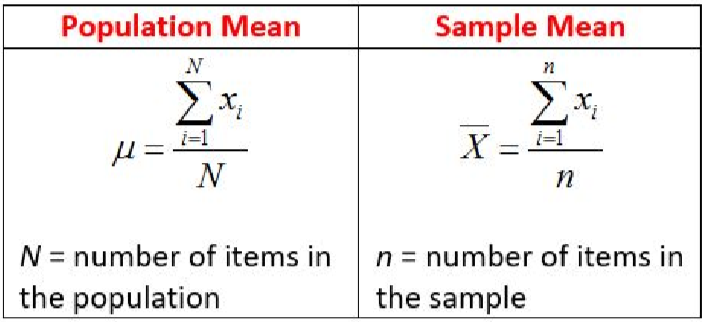
\includegraphics[scale=0.4]{figures/1174057/chapter5/5.png}
				\caption{mean}
				\label{mean}
			\end{figure}

			\begin{figure}[H]
				\centering
				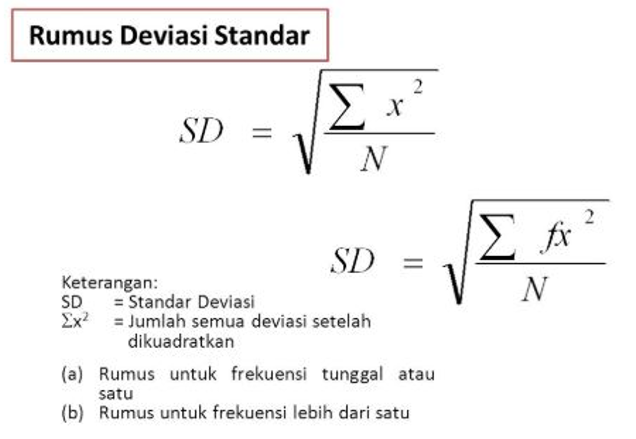
\includegraphics[scale=0.4]{figures/1174057/chapter5/5_1.png}
				\caption{standar deviasi}
				\label{standar deviasi}
			\end{figure}

			\item Jelaskan apa itu skip-gram
			\par Sebuah teknik yang digunakan di area speech processing, dimana n-gram yang dibentuk kemudian ditambahkan juga dengan tindakan “skip” pada token-tokennya. Untuk membentuk k-skip-n-grams, ada dua nilai yang harus didefinisikan, dimana kedua nilai tersebut yaitu k (jumlah kata yang di-skip) dan n (banyak kata dalam n-gram, e.g. bigram (2-gram), trigram (3-gram), dll).
			\begin{figure}[H]
				\centering
				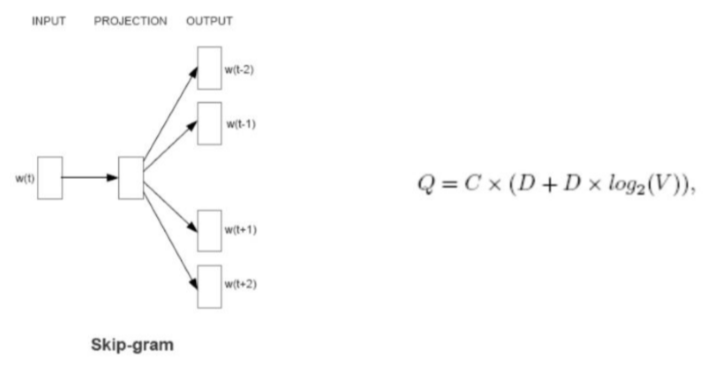
\includegraphics[scale=0.4]{figures/1174057/chapter5/6.png}
				\caption{skip-gram}
				\label{skip-gram}
			\end{figure}		

   		\end{enumerate}

   	\subsection{Praktek}
   		\begin{enumerate}
   			\item mencoba dataset google dan penjelasan vektor dari kata love, faith, fall, sick, clear, shine, bag, car, wash, motor, dan cycle.
   			\begin{itemize}
   				\item berikut merupakan code import gensim digunakan untuk membuat data model atau rangcangan data yang akan di buat. selanjutnya dibuat variabel gmodel yang berisi data vektor negative. selanjutnya data tersebut di load agar data tersebut dapat di tampilkan dan di olah. data tersebut diambil dari GoogleNews-vectors-negative300.bin.
	  			\begin{figure}[H]
					\centering
					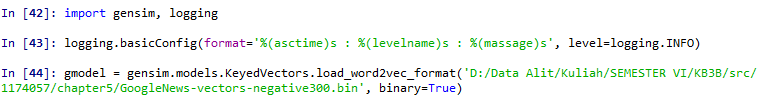
\includegraphics[scale=0.4]{figures/1174057/chapter5/7.PNG}
					\caption{praktek 1}
					\label{praktek 1}
				\end{figure}

				\item berikut merupakan hasil lpengolahan kata love pada data google yang di load tadi. Sehingga memunculkan hasil vektor 300 dimensi untuk kata tersebut.
	  			\begin{figure}[H]
					\centering
					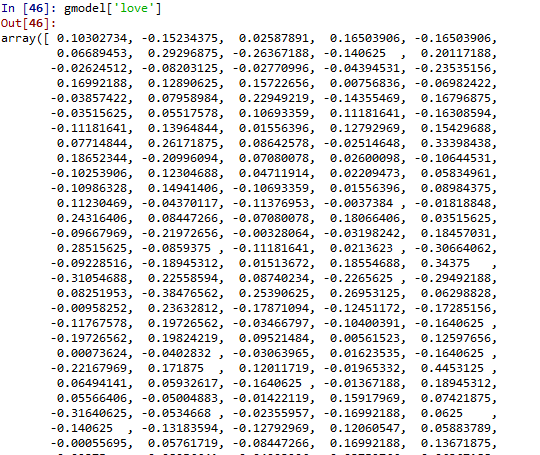
\includegraphics[scale=0.4]{figures/1174057/chapter5/love.PNG}
					\caption{love}
					\label{love}
				\end{figure}

				\item berikut merupakan hasil lpengolahan kata faith pada data google yang di load tadi. Sehingga memunculkan hasil vektor 300 dimensi untuk kata tersebut.
	  			\begin{figure}[H]
					\centering
					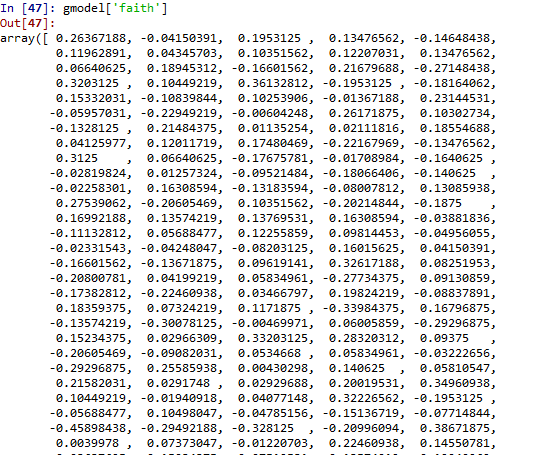
\includegraphics[scale=0.4]{figures/1174057/chapter5/faith.PNG}
					\caption{faith}
					\label{faith}
				\end{figure}

				\item berikut merupakan hasil lpengolahan kata fall pada data google yang di load tadi. Sehingga memunculkan hasil vektor 300 dimensi untuk kata tersebut.
	  			\begin{figure}[H]
					\centering
					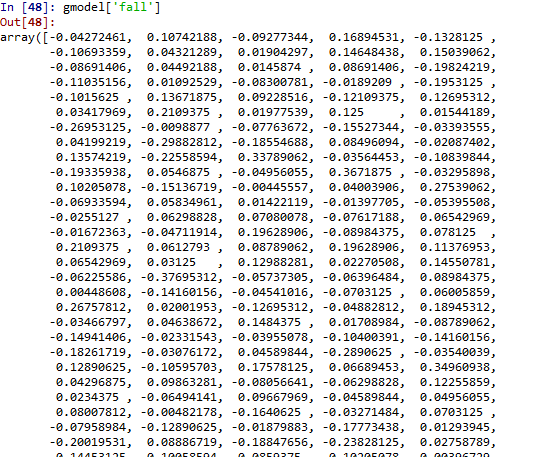
\includegraphics[scale=0.4]{figures/1174057/chapter5/fall.PNG}
					\caption{fall}
					\label{fall}
				\end{figure}

				\item berikut merupakan hasil lpengolahan kata sick pada data google yang di load tadi. Sehingga memunculkan hasil vektor 300 dimensi untuk kata tersebut.
	  			\begin{figure}[H]
					\centering
					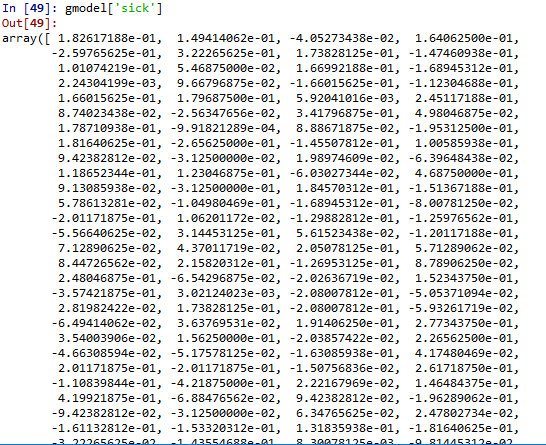
\includegraphics[scale=0.4]{figures/1174057/chapter5/sick.PNG}
					\caption{sick}
					\label{sick}
				\end{figure}

				\item berikut merupakan hasil lpengolahan kata clear pada data google yang di load tadi. Sehingga memunculkan hasil vektor 300 dimensi untuk kata tersebut.
	  			\begin{figure}[H]
					\centering
					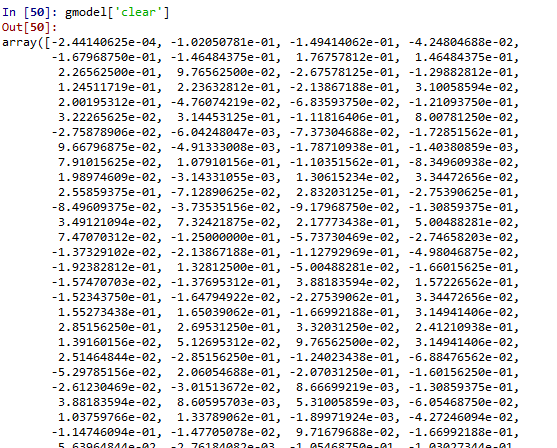
\includegraphics[scale=0.4]{figures/1174057/chapter5/clear.PNG}
					\caption{clear}
					\label{clear}
				\end{figure}

				\item berikut merupakan hasil lpengolahan kata shine pada data google yang di load tadi. Sehingga memunculkan hasil vektor 300 dimensi untuk kata tersebut.
	  			\begin{figure}[H]
					\centering
					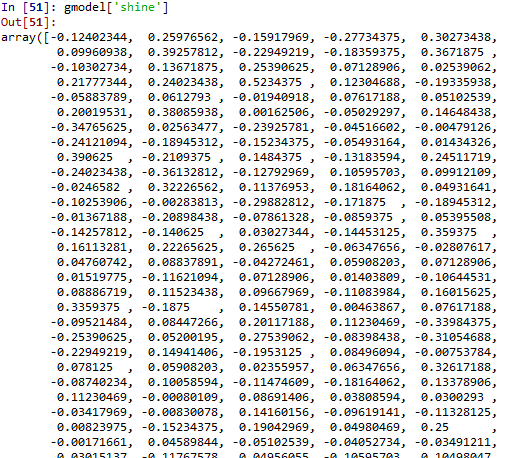
\includegraphics[scale=0.4]{figures/1174057/chapter5/shine.PNG}
					\caption{shine}
					\label{shine}
				\end{figure}

				\item berikut merupakan hasil lpengolahan kata bag pada data google yang di load tadi. Sehingga memunculkan hasil vektor 300 dimensi untuk kata tersebut.
	  			\begin{figure}[H]
					\centering
					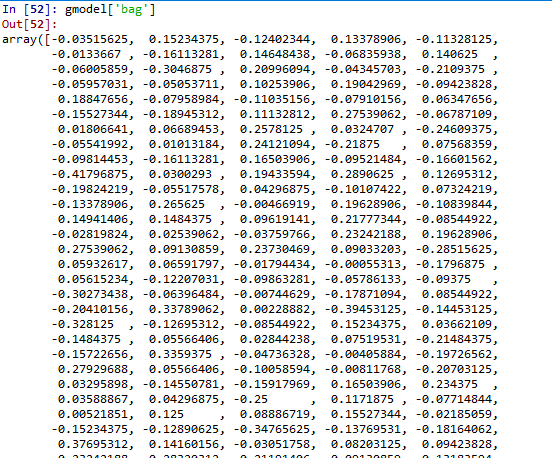
\includegraphics[scale=0.4]{figures/1174057/chapter5/bag.PNG}
					\caption{bag}
					\label{bag}
				\end{figure}

				\item berikut merupakan hasil lpengolahan kata car pada data google yang di load tadi. Sehingga memunculkan hasil vektor 300 dimensi untuk kata tersebut.
	  			\begin{figure}[H]
					\centering
					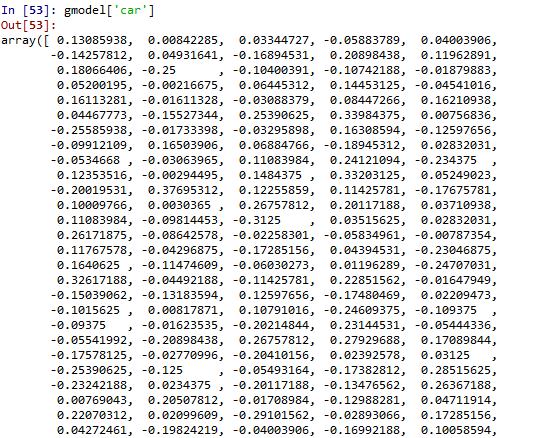
\includegraphics[scale=0.4]{figures/1174057/chapter5/car.PNG}
					\caption{car}
					\label{car}
				\end{figure}

				\item berikut merupakan hasil lpengolahan kata wash pada data google yang di load tadi. Sehingga memunculkan hasil vektor 300 dimensi untuk kata tersebut.
	  			\begin{figure}[H]
					\centering
					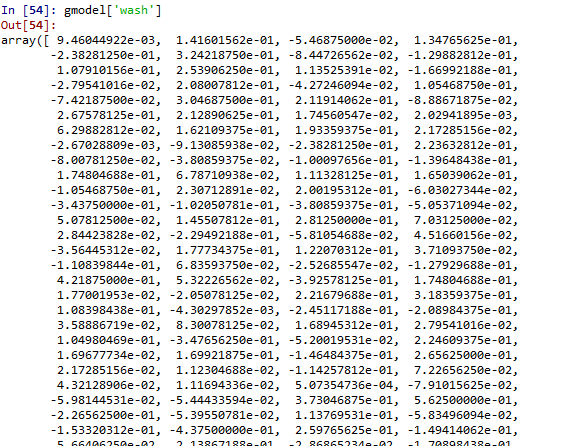
\includegraphics[scale=0.4]{figures/1174057/chapter5/wash.PNG}
					\caption{wash}
					\label{wash}
				\end{figure}

				\item berikut merupakan hasil lpengolahan kata motor pada data google yang di load tadi. Sehingga memunculkan hasil vektor 300 dimensi untuk kata tersebut.
	  			\begin{figure}[H]
					\centering
					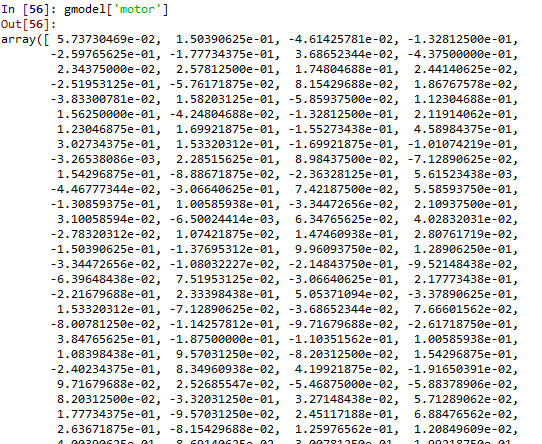
\includegraphics[scale=0.4]{figures/1174057/chapter5/motor.PNG}
					\caption{motor}
					\label{motor}
				\end{figure}

				\item berikut merupakan hasil lpengolahan kata cycle pada data google yang di load tadi. Sehingga memunculkan hasil vektor 300 dimensi untuk kata tersebut.
	  			\begin{figure}[H]
					\centering
					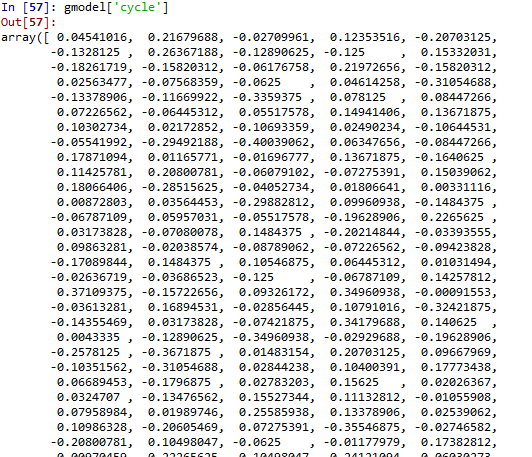
\includegraphics[scale=0.4]{figures/1174057/chapter5/cycle.PNG}
					\caption{cycle}
					\label{cycle}
				\end{figure}

				\item berikut merupakan hasil dari similaritas kata kata yang di olah menjadi matrix tadi adapun persentase untuk perbandingan setiap katanya yaitu 9 persen untuk kata wash dan clear 7 persen untuk kata bag dan love 48 persen untuk kata motor dan car 12 persen untuk kata sick dan faith dan terakhir yaitu 6 persen untuk kata cycle dan shine.
	  			\begin{figure}[H]
					\centering
					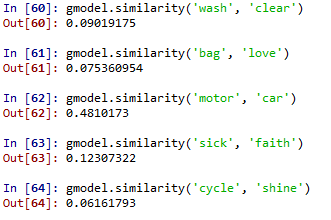
\includegraphics[scale=0.4]{figures/1174057/chapter5/similarity.PNG}
					\caption{similarity}
					\label{similarity}
				\end{figure}				

   			\end{itemize}
   			\item jelaskan dengan kata dan ilustrasi fungsi dari extract words dan PermuteSentences
   			\par Untuk Extract Words berfungsi untuk memecahkan kata menjadi beberapa komponen atau lebih mudahnya kata yang dieksekusi dipecah kemudian dikelompokkan sesuai dengan keinginan
   			\par Pada hasil yang didapatkan untuk contoh ini yaitu terdapat satu kalimat untuk yang terbentuk dari 5 kata. Kata tersebut kemudian di pisahkan menggunakan perintah ( test string.split) kemudian hasil keluarannya akan di print dengan parameter tambahan kata sehingga memberikan penjelasan ataupun tanda yang lebih jelas terhadap perbedaan eksekusi kata ketika masih terangkai dan ketika telah terpecahkan.
	  			\begin{figure}[H]
					\centering
					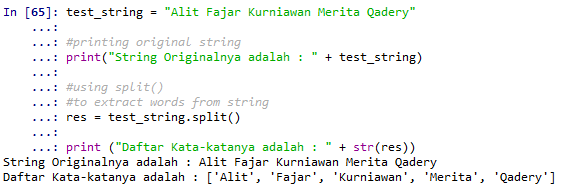
\includegraphics[scale=0.4]{figures/1174057/chapter5/2_1.PNG}
					\caption{praktek2}
					\label{praktek2}
				\end{figure}

			\par Gambar tersebut didalamnya telah mengilustrasikan sebuah kalimat ’Alit Fajar Kurniawan Qadery’ yang akan dipisahkan perkata. Dimana library re (regex module) dan library string di import terlebih dahulu. Kemudian untuk variable out mendefinisikan X untuk mengembalikan string pada objek line yang telah di split yang eksekusi perintah split itu diartikan sebagai (dibagi atau dipisahkan). Kemudian, X dikembalikan berdasarkan jumlah kata yang ada, sehingga muncullah hasil seperti pada gambar yang dijadikansebagai keluaran.
	  			\begin{figure}[H]
					\centering
					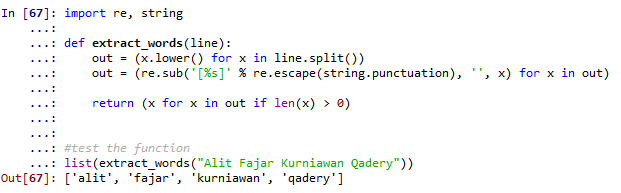
\includegraphics[scale=0.4]{figures/1174057/chapter5/2_2.PNG}
					\caption{praktek2}
					\label{praktek2}
				\end{figure}

			\par PermuteSentences digunakan untuk melakukan pengocokan ( shuffle ataupun random ) pada text yang diiginkan. Pada gambar tersebut mengeluarkan sebuah hasil ( keluaran ) yang telah berupa pengacakan/pengocokan kata/huruf/kalimat yang telah didefinisikan pada perintah untuk dieksekusi. Kata ALIT di random dengan beberapa kali sehingga memberikan hasil yang beragam dimana semuanya berbentuk string dan dieksekusi berupa len. Untuk return dari inputan yang dieksekusi tersebut di definisikan dengan pemanggilan variabel next list.

			\item  Library Gensim TaggedDocument Dan Doc2Vec
			\begin{itemize}
				\item  Gensim TaggedDocument : Tagged Document merupakan class yang digunakan dalam library gensim yang dicontohkan dimana tagged dokument yang ’memisahkan informasi dan struktur dari presentasi’ dengan menggunakan tag . 
				\item Doc2Vec : Untuk membuat representasi numerik dari suatu dokumen, terlepas dari panjangnya. Model doc2vec dapat digunakan dengan cara berikut: untuk pelatihan, diperlukan seperangkat dokumen.

	  			\begin{figure}[H]
					\centering
					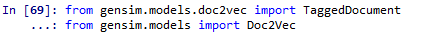
\includegraphics[scale=0.4]{figures/1174057/chapter5/3_1.PNG}
					\caption{praktek3}
					\label{praktek3}
				\end{figure}
			\end{itemize}

			\item menambahkan data training dari file yang dimasukkan kepada variabel dalam rangka melatih model doc2vac.
			\par Penjelasan Untuk Penambahan Data Training : Ada beberapa point penting yang bisa diperhatikan dan dipertimbangkan pada penambahan data yaitu
				\begin{itemize}
					\item Disintegrasi dan Komposisi: Langkah ini melibatkan pemecahan fitur tertentu untuk membangun data pelatihan yang lebih baik untuk model yang Anda pahami lebih komprehensif sehingga menghasilkan hasil yang lebih tepat dan efisien. 
					\item Penskalaan dimana dataset ditempatkan sambil mempertimbangkan kumpulan data linier seperti data bank ataupun data lainnya. 
					\item Kemudian untuk Komposisi: merupakan proses terakhir yang melibatkan penggabungan berbagai fitur menjadi satu fitur untuk mendapatkan data yang lebih akurat atau bermakna.
				\end{itemize}
	  			\begin{figure}[H]
					\centering
					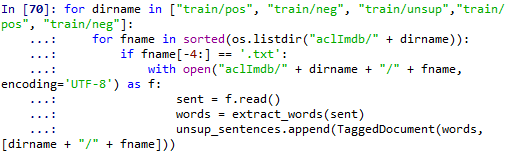
\includegraphics[scale=0.4]{figures/1174057/chapter5/4_1.PNG}
					\caption{praktek4}
					\label{praktek4}
				\end{figure}

			\par penjelasan : direalisasikan pemanggilan directory name ( dirname ) dari file yang akan dieksekusi . Kemudian didefinisikan fname untuk pemberian nama terhadap file tersebut yang akan di urutkan sesuai dengan list dir dengan parameter dirnamenya. Setiap contoh yang diberikan semuanya akan direalisasikan dalam inputan variabel words dengan extract word yang dihubungkan dengan unsup sentences yang mengeksekusi class tagged document. Ketiga gambar tersebut ketika dijalankan tidak terjadi error, maka pengujian atau praktekpun berhasil dilakukan.

			\item pengocokan dan pembersihan data
			\par Pengocokan Data yaitu Melakukan pengacakan terhadap data kemudian nantinya bisa dieksekusi. Kemudian pada setiap eksekusinya akan menghasilkan hasil yang berbeda berdasarkan/berkaitan dengan penerapan mode ( shuffle atau random ) dalam pengeksekusian data. sedangkan Pembersihan Data yaitu Melakukan pengecekan dan pemulihan data.
	  			\begin{figure}[H]
					\centering
					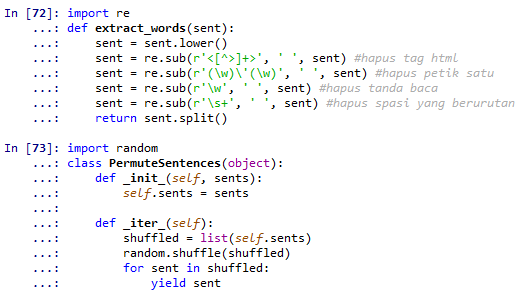
\includegraphics[scale=0.4]{figures/1174057/chapter5/5_P.PNG}
					\caption{praktek5}
					\label{praktek5}
				\end{figure}
			\par penjelasan terjadi pengimportan Library Re. Selanjutnya dilakukan pembuatan fungsi utuk menghapus tag html dan perkocokan ( pengocokan ) . Berkaitan dengan penghapusan tersebut, pada variabel ini terdapat kodingan petik satu yang bisa direalisasikan, tanda baca dan spasi yang berurutan pun ada Selanjutnya yaitu melakukan pengacakan model terhadap data unsupervised learning yang ada, kemudian baru dibuatkan (membuat) modelnya setelah dilakukan pengacakan data yang telah ada sebelumnya.

			\item Mengapa Model Harus Di Save Dan Temporari Training Harus Dihapus
			\par suapaya dalam pengolahan data tidak perlu menjalankan kembali data vektorisasi serta untuk meringankan beban ram. kemudian temporary harus dihapus guna meningkatkan peforma komputer. Model harus di save dikarenakan atau difungsikan untuk mencegah ram pada komputer/laptop tidak terjadi malfuntion ataupun lemot ( loading yang lama ). Kemudian untuk mengapa temporari training harus dihapus dimana digunakan untuk mengosongkan memori sehingga terdapat ruang lebih ataupun lapang sehingga tidak terjadi malfunction pada komputer dll. 
	  			\begin{figure}[H]
					\centering
					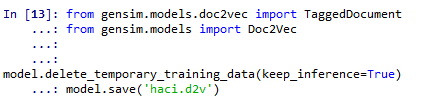
\includegraphics[scale=0.4]{figures/1174057/chapter5/6_1.png}
					\caption{praktek6}
					\label{praktek6}
				\end{figure}

			\par Untuk model gambar pertama diperlihatkan praktek untuk percobaan penghapusan temporary training data dimana apabila parameternya ”keep inference” true maka akan dilakukan penghapusan sesuai dengan perintah yang ada. Kemudian untuk gambar kedua memperlihatkan praktek dari perintah save terhadap sebuah parameter kata yaitu (alit.d2v) yang disimpan berupa INFO berbarengan / disertakan dengan tanggal dan waktu rincinya.

			\item Maksud Dari Infer code
			\par Difungsikan untuk menyimpulkan vector yang mana berhubungan dengan vecktor dokumen baru (pada subjek pengeksekusian). 
			Berdasarkan dari hasil tersebut, kalimat yang dieksekusi yaitu ” saya kamu dia mereka ” dipecah kemudian disimpulkan dimana keluarannya menghasilkan array dengan dtype=float32.

			\item Maksud Dari Cosine similarity
			pengeksekusian dan juga pengujian terhadap model cosine similarity dengan 2 objek kata yaitu ”services sucks 2” memberikan keluaran berupa array sebagai tingkatan kesamaan ataupun perbandingan terhadap kedua kata yang sama tersebut. Hasilnya o.9 sehingga membuktikan tingkat kesamaan yang signifikan diantara keduanya.

			\item Praktek Score Dari Cross Validation
			\par Untuk Praktek dari score cross validation ini akan berpatokan pada perhitungan model clrf, sentvecs, setiments kemudian akan meghitung keakuratan dari data ataupun parameter yang dieksekusi tersebut. Telah dilakukan pengeksekusian untuk pengujian score dari cross validation dengan perhitungan model clrf, sentvecs, setiments sebagai inputan kemudian menghasilkan keluaran ( output ) yang berupa angka dimana akan tersebut diartikan sebagai tingkat keakuratan perhitungan yang terjadi pada inputan yang ada.

   		\end{enumerate}
   	\subsection{Penanganan Error}
